\documentclass[11pt,a4paper]{article}

\usepackage[T1]{fontenc}
\usepackage[utf8]{inputenc}
\usepackage[french]{babel}
\usepackage{geometry}
\usepackage{graphicx}
\usepackage{booktabs}
\usepackage{longtable}
\usepackage{hyperref}
\usepackage{listings}
\usepackage{array}

\geometry{margin=2.5cm}
\hypersetup{colorlinks=true, linkcolor=black, urlcolor=blue}

\lstset{
  basicstyle=\ttfamily\small,
  breaklines=true,
  frame=single,
  columns=fullflexible,
}

\title{PhishGuard\\[0.4em]
\large Plateforme distribuée de détection et qualification d'e-mails de phishing}
\author{Projet de fin de semestre --- Applications réparties et cybersécurité}
\date{\today}

\begin{document}
\maketitle

\begin{abstract}
PhishGuard est une application Python distribuée permettant de signaler des e-mails suspects,
de leur attribuer un score de risque (faible, moyen, élevé) et de conserver un historique
traçable. Quatre services communiquent localement : une passerelle REST, un service
d'authentification, un analyseur gRPC et un service d'audit. Aucune dépendance cloud
n'est requise pour la démonstration.
\end{abstract}

\section{Contexte et objectifs}

Les campagnes de phishing exploitent l'urgence, l'usurpation de marque et des liens
trompeurs. L'objectif n'est pas de produire un antivirus complet, mais une plateforme
pédagogique qui centralise les signalements, applique des règles explicables et journalise
les actions sensibles.

Fonctions couvertes :
\begin{itemize}
  \item authentification avec rôles (administrateur, analyste, utilisateur) ;
  \item soumission et validation d'un e-mail suspect ;
  \item analyse heuristique et score de risque ;
  \item consultation et recherche dans l'historique ;
  \item audit des connexions et soumissions.
\end{itemize}

\section{Architecture distribuée}

La figure~\ref{fig:archi} présente l'architecture retenue. Le client web contacte
uniquement l'API Gateway (port 8000). Celle-ci délègue la vérification d'identité
au AuthService (HTTP/JSON), l'analyse au AnalysisService (gRPC/Protobuf) et
l'enregistrement des événements au AuditService (HTTP/JSON).

\begin{figure}[htbp]
  \centering
  % Exporter schema.pdf depuis docs/architecture/schema.svg (voir docs/architecture/README.md)
  \IfFileExists{architecture/schema.pdf}{%
    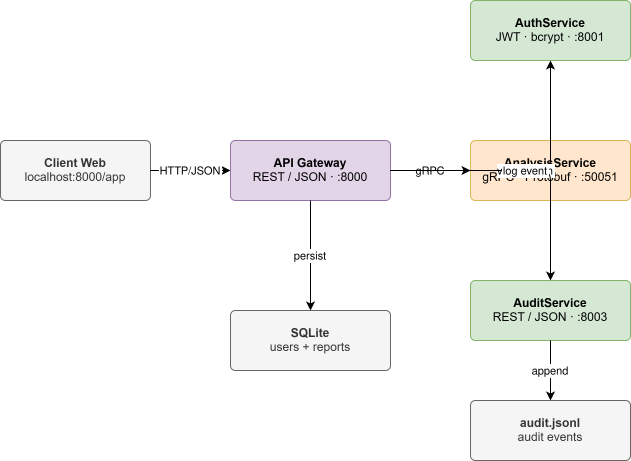
\includegraphics[width=0.95\textwidth]{architecture/schema.pdf}%
  }{%
    \fbox{\parbox{0.9\textwidth}{\centering\vspace{2cm}
    Placeholder --- compiler après export de\\
    \texttt{docs/architecture/schema.pdf}\vspace{2cm}}}%
  }
  \caption{Architecture PhishGuard (Client, Gateway, Auth, Analysis gRPC, Audit, SQLite/JSONL)}
  \label{fig:archi}
\end{figure}

\begin{table}[htbp]
  \centering
  \caption{Services et protocoles}
  \begin{tabular}{@{}llll@{}}
    \toprule
    Service & Port & Protocole & Rôle \\
    \midrule
    API Gateway & 8000 & REST / JSON & Entrée unique, orchestration, stockage signalements \\
    AuthService & 8001 & REST / JSON & Login, JWT, rôles \\
    AnalysisService & 50051 & gRPC / Protobuf & Scoring heuristique \\
    AuditService & 8003 & REST / JSON & Logs d'audit (JSONL) \\
    \bottomrule
  \end{tabular}
\end{table}

Stockage local : SQLite (\texttt{data/phishguard.db}) pour utilisateurs et signalements ;
fichier \texttt{audit\_service/data/audit.jsonl} pour l'audit.

\section{Fonctionnement d'une soumission}

Séquence typique lors d'un signalement :
\begin{enumerate}
  \item le client envoie un JWT dans l'en-tête \texttt{Authorization} ;
  \item la Gateway appelle AuthService pour valider le token et le rôle ;
  \item le corps de la requête est validé (Pydantic) puis transmis en gRPC à AnalysisService ;
  \item le score et les justifications sont renvoyés au client ;
  \item le signalement est persisté en SQLite et un événement d'audit est écrit.
\end{enumerate}

Timeouts configurés sur les appels HTTP (3--10\,s) et gRPC (10\,s). En cas d'indisponibilité
d'un service, la Gateway renvoie des codes \texttt{502}/\texttt{503}/\texttt{504} avec un
message générique.

\section{Moteur d'analyse}

AnalysisService applique un score cumulatif (0--100) basé sur des règles lisibles :
langage urgent ou manipulateur, TLD suspects, URLs en IP, raccourcisseurs, homoglyphes,
écart entre domaine expéditeur et liens, pièces jointes annoncées, corps quasi vide, etc.

Seuils :
\begin{itemize}
  \item \textbf{faible} : score $< 30$ ;
  \item \textbf{moyen} : $30 \leq$ score $< 60$ ;
  \item \textbf{élevé} : score $\geq 60$.
\end{itemize}

Chaque règle déclenchée produit une justification textuelle retournée au client.

\section{Cybersécurité}

\subsection{Contrôles implémentés}

\begin{itemize}
  \item mots de passe hashés (bcrypt), jamais stockés en clair ;
  \item JWT signé (HS256) avec expiration ; refresh token séparé ;
  \item validation stricte des entrées et limites de taille ;
  \item contrôle des rôles (admin / analyst / user) ;
  \item rate limiting (30 requêtes/min/IP) ;
  \item échanges d'analyse en Protobuf (pas de pickle) ;
  \item logs structurés côté serveur, erreurs non bavardes côté client.
\end{itemize}

\subsection{Tableau des menaces principales}

{\small
\begin{longtable}{@{}p{2.6cm}p{3.2cm}p{2.2cm}p{5.2cm}@{}}
\toprule
Menace & Description & Composant & Protection \\
\midrule
\endhead
Usurpation d'identité & Token JWT volé ou forgé & Gateway & Vérification JWT via AuthService ; expiration 60 min \\
Falsification & Payload ou champs injectés & Gateway & Validation Pydantic ; plafonds taille \\
Répudiation & Nier login ou soumission & Audit & Événements JSONL horodatés (login, soumission) \\
Divulgation & Fuites dans les erreurs & Tous & Messages génériques au client \\
DoS & Flood de requêtes & Gateway & Rate limit ; caps payload \\
Élévation de privilèges & Accès admin illégitime & Gateway & \texttt{require\_admin} sur endpoints sensibles \\
Injection & Contenu malveillant & Analysis, DB & Pydantic ; SQL paramétré \\
Rejeu de token & Token intercepté réutilisé & Auth & Claim \texttt{exp} ; type refresh séparé \\
Désérialisation unsafe & Objet Python malveillant & gRPC & Protobuf uniquement \\
Fuite credentials & Secrets dans le dépôt & Git & \texttt{.env} ignoré ; bcrypt \\
Brute force & Deviner un mot de passe & Auth & Rate limit ; erreur générique \\
\bottomrule
\end{longtable}
}

\section{Démonstration}

\subsection{Installation et lancement}

\begin{lstlisting}[language=bash]
python -m venv .venv && source .venv/bin/activate  # Windows: .venv\Scripts\activate
pip install -r requirements.txt
cp .env.example .env   # modifier JWT_SECRET
python setup_users.py
# lancer auth_service, audit_service, analysis_service, api_gateway
\end{lstlisting}

Interface : \url{http://localhost:8000/app/index.html}

\subsection{Jeu de données}

Cinq fichiers JSON dans \texttt{docs/demo/} simulent des cas suspects ou légitimes
(voir \texttt{docs/demo/README.md}). Exemple : \texttt{phishing\_credential\_harvest.json}
(demande urgente de renouvellement + raccourcisseur) doit produire un risque élevé.

\subsection{Scénario oral}

\begin{enumerate}
  \item connexion analyste ;
  \item soumission d'un e-mail de test ;
  \item observation du score et des justifications ;
  \item consultation de l'historique avec filtres ;
  \item refus d'accès sans token ;
  \item connexion admin et lecture du journal d'audit ;
  \item arrêt d'AnalysisService pour illustrer une erreur gérée (502/503).
\end{enumerate}

\section{Choix techniques et limites}

\textbf{JSON vs Protobuf :} REST/JSON pour l'API publique (simplicité, débogage) ;
Protobuf pour Gateway$\rightarrow$Analysis (contrat typé, pas de désérialisation Python arbitraire).

\textbf{Limites :} moteur heuristique sans ML ; rate limit en mémoire (non partagé entre
instances) ; schéma d'architecture à finaliser dans \texttt{docs/architecture/}.

\section{Conclusion}

PhishGuard répond aux exigences du projet : architecture répartie réelle, analyse
explicable, sécurité by design et démonstration locale. Les livrables (code, README,
schéma, rapport, jeu de données, tableau des menaces) sont regroupés dans le dépôt
GitHub sous \texttt{docs/}.

\end{document}
